\documentclass[margin,line]{resume}
\usepackage{amsmath}

\usepackage[latin1]{inputenc}
\usepackage[english]{babel}
\usepackage[T1]{fontenc}
\usepackage{graphicx,wrapfig}
\usepackage{url}

\usepackage[colorlinks=true, a4paper=true, pdfstartview=FitV,
linkcolor=blue, citecolor=blue, urlcolor=blue]{hyperref}
\pdfcompresslevel=9


\begin{document}

~
\vspace{-2.0cm}

{\sc \Large Curriculum Vitae ~~~~~~~~~~~~~~~~~~~~~~~~~~~~~~~~~~~~~~~~~~~~ \scriptsize update \today}
\begin{resume}
    \vspace{0.5cm}
    
    % Picture:
%    \begin{wrapfigure}{R}{0.3\textwidth}
%        \vspace{-1cm}
%       \begin{center}
%       	\hspace{-0.5cm}
%       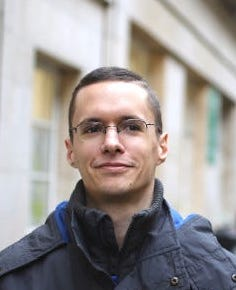
\includegraphics[width=0.25\textwidth]{ferraris_s}
%       \end{center}
%     \vspace{-1cm}
%    \end{wrapfigure}
    
    \section{\mysidestyle Contacts}
    
    Sebastiano Ferraris 
    
    +44 7756891803
    
    \href{mailto:sebastiano.ferraris@gmail.com}{sebastiano.ferraris@gmail.com}

    $\triangleright$ \href{http://www.github.com/SebastianoF}{GitHub}\\
    $\triangleright$ \href{https://www.researchgate.net/profile/Sebastiano_Ferraris}{ResearchGate}\\
    $\triangleright$ \href{https://www.linkedin.com/in/ibis-redibis/}{LinkedIn}\\
    $\triangleright$ \href{https://scholar.google.com/citations?user=1tAeAI0AAAAJ&hl=en}{Google Scholar}\\
    $\triangleright$ \href{https://geospatial.netlify.app/posts/}{Blog}

%~
\section{\mysidestyle Studies \\ and \\ Works}


{\bf Data Scientist - \href{https://www.generalsystem.com/}{General System} - $2020$-Present} 
\vspace{0.1cm}
\begin{itemize}
    \item[] \hspace{-1.0cm} Geospatial data Science Services: Startup in stealth mode until April 2022
    \item[$\triangleright$] Developing high standard prototypes, and maintaining their cloud deployment.
    \item[$\triangleright$] Collaborating with clients and domain experts to quickly and iteratively integrate feedback into prototypes.
    \item[$\triangleright$] Managing prototypes handover to production and DevSecOps teams.
    \item[$\triangleright$] Presentation of experimental and algorithmic research to stakeholders.
    \item[$\triangleright$] Contributing to the company blog to build a community around the topics of geospatial data science.
\end{itemize}


{\bf Algorithm Engineer - \href{https://www.paceup.com/}{Pace Revenue Management} - $2019$-$2020$} 
\vspace{0.1cm}
\begin{itemize}
    \item[] \hspace{-1.0cm} Dynamic pricing for the hospitality industry
    \item[$\triangleright$] Simulation and Validation team, aimed at validate and test the python-based ETL pipeline and the core algorithms.
    \item[$\triangleright$] Production code maintenance and new features integration.
\end{itemize}


{\bf Back End Developer - \href{https://www.thoughtmachine.net/}{Thought Machine} - $2018$-$2019$}
\vspace{0.1cm}
\begin{itemize}
    \item[] \hspace{-1.0cm} Cloud native core banking
    \item[$\triangleright$] State-of-the-art infrastructure technologies to deploy microservices in a cloud-agnostic environment: Python, Go, Docker, Kubernetes, and derived customisations.
    \item[$\triangleright$] Maintenance and improvement of the Thought Machine's CI/CD and release pipelines.
\end{itemize}


{\bf MRes + PhD in Medical Image analysis - \href{https://www.ucl.ac.uk/medical-physics-biomedical-engineering/study/postgraduate-research/medical-imaging-mres-mphilphd}{UCL CDT} - $2015$-$2019$} 
\vspace{0.1cm}
\begin{itemize}
    \item[] \hspace{-1.0cm} Research Student
    \item[$\triangleright$] Pre-clinical trial on pre-term birth steroids administration in a multi-disciplinary international research team.
    \item[$\triangleright$] Published 7 peer reviewed papers on the topic of diffeomorphic image registration and ML for automated MRI segmentation.
    \item[$\triangleright$] Recipient of best young scientist poster award at the first Workshop on Assistive Technology for Fetal Therapy and Surgery.
    \item[$\triangleright$] Reproducible research advocate: open sourced 12 Python libraries, and one micro MRI dataset.
\end{itemize}


{\bf Industrial Simulation Modeller - \href{https://www.simtec-group.eu/it/}{SimTec} - $2013$-$2014$}
\vspace{0.1cm}
\begin{itemize}
    \item[] \hspace{-1.0cm} Automotive industry, process and flow simulation
    \item[$\triangleright$] Material flow simulation models to estimate efficiency, remove bottlenecks, dimension buffers and support plant layout design for a range of clients in Italy and Germany.
    \item[$\triangleright$] In house algorithms development for the internal and external logistics of assembly parts, from plant's gate to assembly line. 
    \item[$\triangleright$] Presented at the first annual Tecnomatix Plant Simulation User Conference in Stuttgart.
\end{itemize}


{\bf Algorithms developer - \href{https://www.tc-web.it}{TcWeb} - $2011$}
\vspace{0.1cm}
\begin{itemize}
    \item[] \hspace{-1.0cm} Web development and technology consulting
    \item[$\triangleright$] Term contracts as Junior Developer in Java, Java J2EE,
    Struts 2, Uml, Android app development. 
    \item[$\triangleright$] Algorithms developer: prototyped and implemented a generalised Hungarian Algorithm to parse newspapers' pages.
\end{itemize}


{\bf Bachelor + Master degree in Mathematics - \href{https://en.unito.it/}{UNITO} - $2006$-$2014$}
\vspace{0.1cm}
\begin{itemize}
    \item[] \hspace{-1.0cm} Universita' degli Studi di Torino
    \item[$\triangleright$] Graduated in mathematics with specialisation in Computational Algebra and Geometry.
    \item[$\triangleright$] Master of Science in Mathematics with specialisation in Geometry and a thesis about a new application of the Winograd Transform.
\end{itemize}


\section{\mysidestyle Volunteering}

{\bf Maths tutoring programme} -  \href{https://actiontutoring.org.uk/}{Action Tutoring} - $2017$-$2018$ and $2019$-$2020$ \\
At the City of London Academy Highgate Hill College. 

\section{\mysidestyle Skills}
Research, data science, algorithms development and prototypes productionisation, pragmatic and goal oriented, mutlidisciplinary collaborations. \\ \\ 
\textbf{Prototypes:} Python, Streamlit (Jupyter, Numpy, scipy, Scikit-Learn, Matplotlib, Pandas, geopandas). Also: Matlab, Maple, PariGP.\\ \\
\textbf{Production:} FastAPI, OOProgramming, PostrgreSQL. Also: C$++$, Java, Rust, Go, Kubernetes, Helm. \\ \\
\textbf{Methods:} AGILE, jira, phabricator, git, github, gitlab, Docker. CI/CD automation, unit testing, integration testing, test driven development. Code reproducibility, static documentation, dev-prod parity.\\ \\ 

\end{resume}
\end{document}
